\documentclass[review]{elsarticle}
%-----------------------------------------------------

\usepackage{amsmath}
\usepackage{graphicx}

\graphicspath{{./figs/}}

\newcommand{\ihat}{\boldsymbol{\hat{\textbf{\i}}}}
\newcommand{\jhat}{\boldsymbol{\hat{\textbf{\j}}}}
\newcommand{\roughly}{{\raise.17ex\hbox{$\scriptstyle\sim$}}}
\newcommand{\dmax}{d_\text{max}}
\newcommand{\dmin}{d_\text{min}}

%-----------------------------------------------------

\makeatletter
\renewcommand{\fnum@figure}{Figure 2}
\makeatother

\thispagestyle{empty}

\begin{document}
\allowdisplaybreaks

\begin{figure}[ht]
\centering
%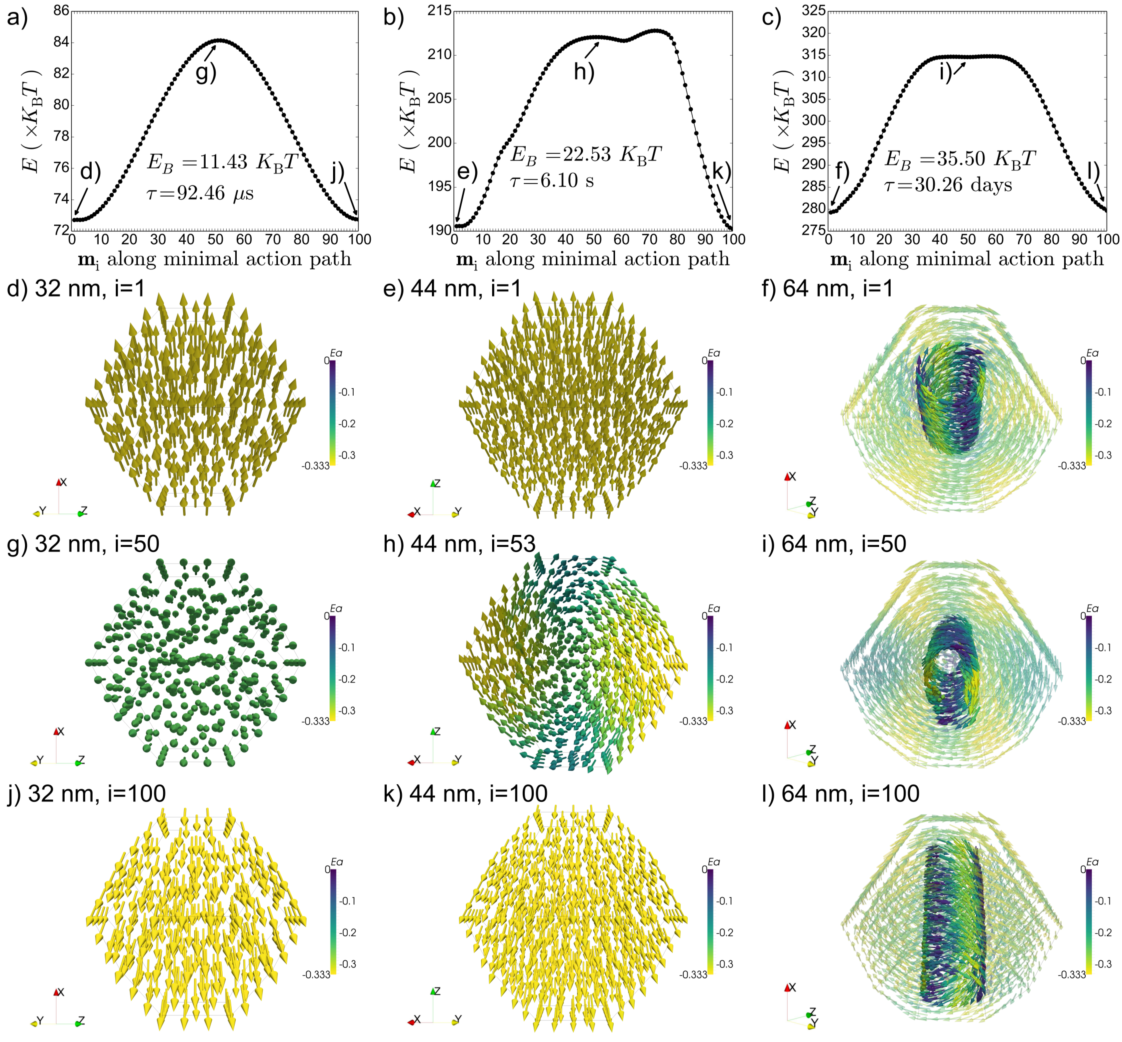
\includegraphics[width=\textwidth]{Figure_07_HR.pdf}
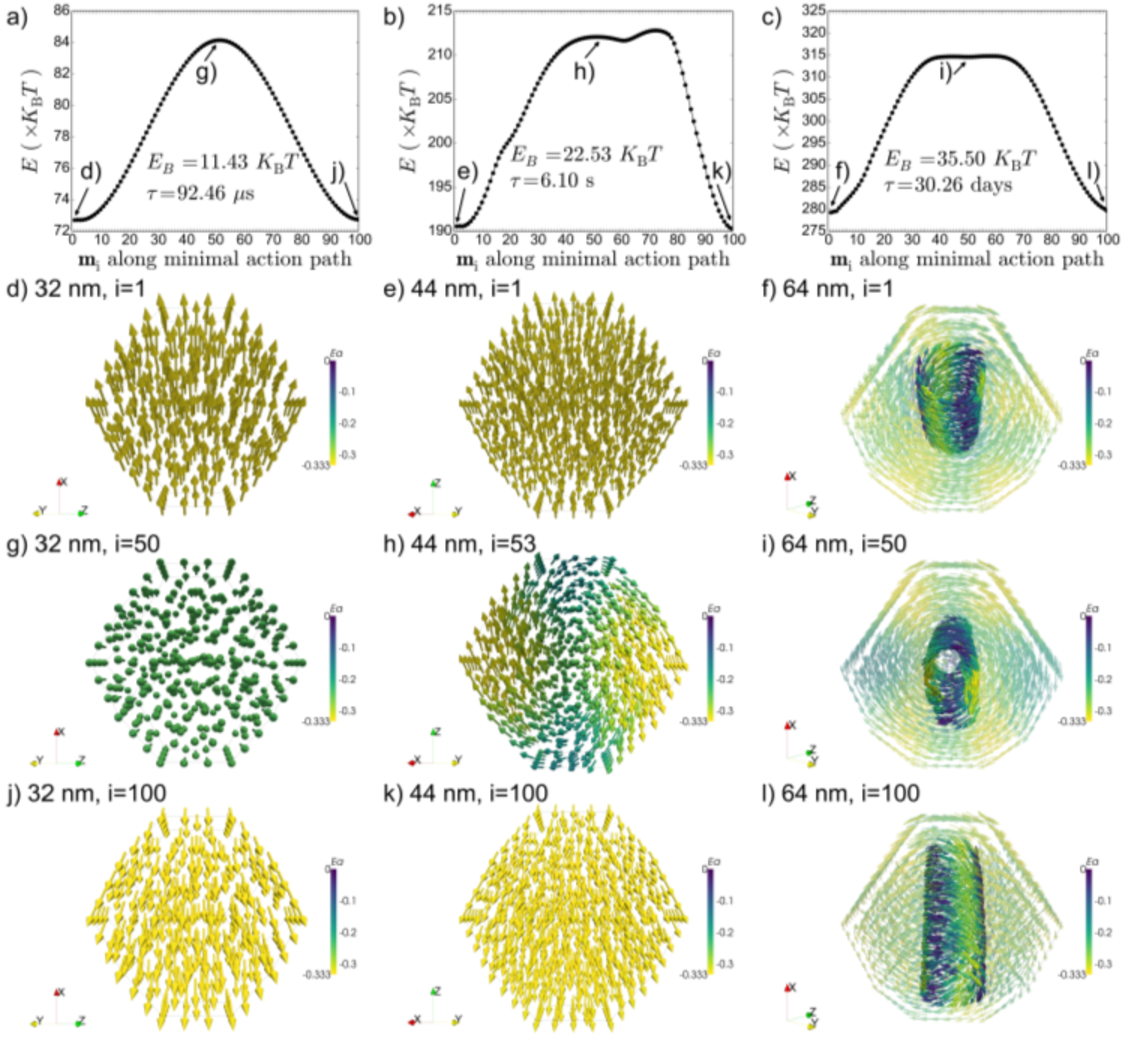
\includegraphics[width=\textwidth]{Figure_07.pdf}
\caption{Typical action-minimising paths. The regular truncated octahedra illustrate the typical AMPs found for all the (truncated) octahedral shapes. Well below the SD--PSD threshold the AMP between SD configurations is a coherent rotation (left column). The energy along the AMP is a single bump (a) and the energy barrier is an intermediate-aligned SD state (d). At sizes just below the SD--PSD threshold the AMP is still between SD states, but via a curling mode (vortex nucleation) (center column). Starting from SD (e), a vortex is nucleated (h) then unwinds to an intermediate-aligned SD state which has the highest energy along the AMP (not shown). Then, the final SD state (k) is reached via coherent rotation. This makes the energy along the AMP more complex and asymmetric (b). Well above the SD--PSD threshold, once the EAV has the lowest energy, the AMP is via a structured rotation of the vortex core (right column). The transition is between two EAVs with the same chirality (f, l) as a change of chirality produces prohibitively large energy barriers. In the AMP there is an IAV sitting in its own shallow LEM (i). The energy barrier is the one that separates the EAVs from the IAV. However, as the grain grows, the IAV LEM becomes more shallow and the energy along the AMP flattens (c). Colour represents the MCA energy normalised by $|K_1|$. The energies along the AMPs are plotted in units of $K_\text{B}T$, with $T=300\,\text{K}$. The left column of Video 1 (supplementary material) shows these transitions.}
\label{fig7}
\end{figure}

\end{document}